\documentclass[12pt,letterpaper]{article}

\usepackage{xr-hyper}       % cross-referencing (must be loaded before hyperref)
\usepackage[hypertexnames=false, draft]{hyperref}
\usepackage{amsmath}
\usepackage{graphicx}
\usepackage{enumerate}
\usepackage{natbib}

% Custom packages
\usepackage{amsthm, amssymb}
\usepackage{booktabs}       % professional-quality tables
\usepackage{algorithm}      % algorithm environment
\usepackage{algpseudocode}
\usepackage{multirow}
\usepackage{sectsty}
\usepackage{tabularx}
\usepackage{tikz}           % vector graphics
\usepackage{bm}             % bold math symbols
\usepackage{xcolor}
\usepackage{microtype}
\usepackage{import}
\usepackage{titling}
\usetikzlibrary{arrows, backgrounds, patterns, matrix, shapes, fit, 
  calc, shadows, plotmarks}

\graphicspath{{./app-figures/}}

% Custom commands
\let\oldvec\vec
\renewcommand\vec{\bm}
\newcommand{\simfn}{\mathtt{sim}} % similarity function
\newcommand{\truncsimfn}{\underline{\simfn}} % truncated similarity function
\newcommand{\blockfn}{\mathtt{BlockFn}} % blocking function
\newcommand{\distfn}{\mathtt{dist}} % distance function
\newcommand{\valset}{\mathcal{V}} % attribute value set
\newcommand{\entset}{\mathcal{R}} % set of records that make up an entity
\newcommand{\partset}{\mathcal{E}} % set of entities that make up a partition
\newcommand{\1}[1]{\mathbb{I}\!\left[#1\right]} % indicator function
\newcommand{\euler}{\mathrm{e}} % Euler's constant
\newcommand{\dblink}{\texttt{\upshape \lowercase{d-blink}}} % Name of scalable Bayesian ER model
\newcommand{\blink}{\texttt{\upshape \lowercase{blink}}} % Name of original Bayesian ER model
\def\spacingset#1{\renewcommand{\baselinestretch}%
  {#1}\small\normalsize} \spacingset{1}

\renewcommand{\theequation}{S\arabic{equation}}
\renewcommand{\thefigure}{S\arabic{figure}}
\renewcommand{\thetable}{S\arabic{table}}
\renewcommand{\thealgorithm}{S\arabic{algorithm}}

\newtheorem*{remark}{Remark}
\newtheorem{proposition}{Proposition}
\newtheorem*{definition}{Definition}

% DON'T change margins - should be 1 inch all around.
\addtolength{\oddsidemargin}{-.5in}%
\addtolength{\evensidemargin}{-.5in}%
\addtolength{\textwidth}{1in}%
\addtolength{\textheight}{1.3in}%
\addtolength{\topmargin}{-.8in}%

\externaldocument{unblinded-paper}

\title{\bf Appendices for ``d-blink: Distributed End-to-End Bayesian Entity Resolution''}
\author{Neil G.~Marchant\textsuperscript{a} \and
	Andee Kaplan\textsuperscript{b} \and 
	Daniel N.~Elazar\textsuperscript{c} \and
	Benjamin I.~P.~Rubinstein\textsuperscript{a} \and 
	Rebecca C.~Steorts\textsuperscript{d}}
\date{
	\textsuperscript{a}School of Computing and Information Systems, University 
	of Melbourne\\
	\textsuperscript{b}Department of Statistics, Colorado State University\\
	\textsuperscript{c}Methodology Division, Australian Bureau of Statistics\\
	\textsuperscript{d}Department of Statistical Science and Computer Science, Duke University\\Principal Mathematical Statistician, United States Census Bureau\\[2ex]
	\today}

\begin{document}
\maketitle

\newpage

\appendix
\section{Derivation of the posterior distribution}
\label{app-sec:full-posterior}
Here we sketch the derivation of the joint posterior distribution over the 
unobserved variables conditioned on the observed record attributes 
$\vec{X}^{(o)}$, which is given in 
Equation~\ref{eqn:partitioned-posterior} of the paper.
First we read the factorization off the plate diagram in 
Figure~\ref{fig:plate-diagram}, together with the conditional dependence 
assumptions detailed in Section~\ref{sec:model-specification} of the paper.
We obtain the following expression, up to a normalisation constant:
\begin{equation*}
\begin{split}
& p(\vec{\Gamma}, \vec{\Lambda}, \vec{Y}, \vec{Z}, \vec{\Theta}, \vec{X}^{(m)}|\vec{X}^{(o)}, \vec{O}) \propto 
  \prod_{e,a} p(y_{ea}|\phi_{a}) 
  \times \prod_{t,a} p(\theta_{ta}|\alpha_{a}, \beta_{a}) \\
& \quad {} \times 
  \prod_{t,r} \Big\{ p(\gamma_{tr}|\vec{Y})p(\lambda_{tr}|\gamma_{tr}, \vec{Y}) 
  \prod_{a} p(z_{tra}|\theta_{ta}) \Big\} 
  \times \prod_{\substack{t,r,a\\o_{tra}=1}} p(x_{tra}|z_{tra}, \lambda_{tr}, y_{\lambda_{tr}a}) \\
& \qquad {} \times 
  \prod_{\substack{t,r,a\\o_{tra}=0}} p(x_{tra}|z_{tra}, \lambda_{tr}, y_{\lambda_{tr}a}).
\end{split}
\end{equation*}
Ideally, we'd like to marginalize out all variables except $\vec{\Lambda}$ and 
$\vec{Y}$ (the variables of interest), however this is not tractable 
analytically.
Fortunately, we can marginalize out the missing record attributes 
$\vec{X}^{(m)}$ which yields Equation~\ref{eqn:partitioned-posterior} 
from the paper:
\begin{equation*}
\begin{split}
& p(\vec{\Gamma}, \vec{\Lambda}, \vec{Y}, \vec{Z}, \vec{\Theta}|\vec{X}^{(o)}, \vec{O}) \propto \prod_{e,a} p(y_{ea}|\phi_{a}) 
  \times \prod_{t,a} p(\theta_{ta}|\alpha_{a}, \beta_{a}) \\
& \quad {} \times 
  \prod_{t,r} \Big\{ p(\gamma_{tr}|\vec{Y})p(\lambda_{tr}|\gamma_{tr}, \vec{Y}) 
  \prod_{a} p(z_{tra}|\theta_{ta}) \Big\} 
  \times \prod_{\substack{t,r,a\\o_{tra}=1}} p(x_{tra}|z_{tra}, \lambda_{tr}, y_{\lambda_{tr}a}).
\end{split}
\end{equation*}

We can expand this further by substituting the conditional distributions 
given in Section~\ref{sec:model-specification} of the paper.
This yields:
\begin{equation}
\begin{split}
& p(\vec{\Gamma}, \vec{\Lambda}, \vec{Y}, \vec{Z}, \vec{\Theta}|\vec{X}^{(o)}, \vec{O}) \propto 
  \prod_{e,a} \phi_{a}(y_{ea}) \times \prod_{t,a} \theta_{ta}^{\alpha_{a} - 1} (1 - \theta_{ta})^{\beta_{a} - 1} \\
& \quad {} \times \prod_{t,r} \Big\{ \1{\lambda_{tr} \in 
  \partset_{\gamma_{tr}}(\vec{Y})} \prod_{a} \theta_{ta}^{z_{tra}} (1 - \theta_{ta})^{1-z_{tra}} \Big\} \\
& \mspace{40mu} {} \times  \prod_{\substack{t,r,a\\o_{tra}=1}} 
  \Big\{ (1 - z_{tra}) \1{x_{tra} = y_{\lambda_{tr}a}} 
  + z_{tra} \, \psi_{a}(x_{tra}|y_{\lambda_{tr}a}) \Big\}.
\end{split}
\label{app-eqn:expanded-posterior}
\end{equation}

\section{Equivalence of \texorpdfstring{\dblink}{d-blink} and \texorpdfstring{\blink}{blink}}
In this section, we present proofs of 
Propositions~\ref{thm:sim-dist-equiv} and~\ref{thm:posterior-equiv}, 
which show that the inferences we obtain from \dblink\ are equivalent to those 
we would obtain from \blink\ under certain conditions.

\subsection{Proof of Proposition~\ref{thm:sim-dist-equiv}: equivalence of 
distance\slash similarity representations}
\label{app-sec:proof-sim-dist-equiv}
It is straightforward to show that $\simfn$ as defined in 
Equation~\ref{eqn:simfn-distfn-correspondence} of the paper satisfies 
the requirements of Definition~\ref{def:attribute-sim-measure}.
All that remains is to show that the two parameterizations of the distortion 
distribution $\psi_{a}$ are equivalent.
Beginning with $\psi_{a}$ as parameterized in \blink, we substitute 
Equation~\ref{eqn:simfn-distfn-correspondence} and observe that
\begin{equation*}
\psi_{a}(v|w) \propto \phi_{a}(v) \euler^{-\distfn_{a}(v, w)} 
   = \phi_{a}(v) \euler^{d_\mathrm{max;a} + \simfn_{a}(v, w)} 
   \propto \phi_{a}(v) \euler^{\simfn_{a}(v, w)}.
\end{equation*}
This is identical to our parameterization in 
Equation~\ref{eqn:distortion-dist}. \qed

\subsection{Proof of Proposition~\ref{thm:posterior-equiv}: equivalence of 
\texorpdfstring{\dblink}{d-blink} and \texorpdfstring{\blink}{blink}}
\label{app-sec:proof-posterior-equiv}
Given that 
\begin{itemize}
  \item Proposition~\ref{thm:sim-dist-equiv} holds, 
  \item the distortion hyperparameters are the same for all attributes, and 
  \item all record attributes are observed,
\end{itemize}
the only factor in the posterior that differs from \blink\ is:
\begin{equation}
\prod_{t,r} p(\lambda_{tr}| \gamma_{tr}, \vec{Y}) 
  p(\gamma_{tr}|\vec{Y}).
\label{app-eqn:posterior-part-factor}
\end{equation}
Substituting the density for the conditional distributions 
for a single $t,r$ factor yields:
\begin{equation*}
p(\lambda_{tr}|\gamma_{tr},\vec{Y}) p(\gamma_{tr}|\vec{Y})
= \frac{\1{\lambda_{tr} \in \partset_{\gamma_{tr}}(\vec{Y})}}
{|\partset_{\gamma_{tr}}(\vec{Y})|} 
\times \frac{|\partset_{\gamma_{tr}}(\vec{Y})|}{E} = \frac{1}{E} \1{\lambda_{tr} \in \partset_{\gamma_{tr}}(\vec{Y})}.
\end{equation*}
Putting this in Equation~\ref{app-eqn:posterior-part-factor} and 
marginalizing over $\vec{\Gamma}$ we obtain:
\begin{equation*}
\prod_{t,r} \sum_{\gamma_{tr} = 1}^{B} p(\lambda_{tr}|\gamma_{tr},\vec{Y}) p(\gamma_{tr}|\vec{Y}) 
= \prod_{t,r} \frac{1}{E} \sum_{\gamma_{tr} = 1}^{B} \1{\lambda_{tr} \in \partset_{\gamma_{tr}}(\vec{Y})} 
= \prod_{t,r} \frac{1}{E} \1{\lambda_{tr} \in \{1,\ldots,E\}},
\end{equation*}
which is the factor that appears in the posterior for \blink. \qed

\section{Splitting rules for the \textit{k}-d tree blocking function}
\label{app-sec:splitting-rules}
In Section~\ref{sec:kd} of the paper we outline a blocking function inspired 
by $k$-d trees.
When inserting a node in the tree, we require a splitting rule that partitions 
the input set of values.
In ordinary $k$-d trees, the median is often used for this purpose, 
however it is not appropriate for the discrete input sets that we 
encounter.
As a result, we propose the following alternative splitting rules:
\begin{enumerate}
  \item \emph{Ordered median.}
  This rule is appropriate if the set of input attribute 
  values is large and\slash or has a natural ordering.
  If there is no natural ordering, an artificial ordering 
  must be applied (e.g. lexicographic ordering).
  The splitting rule is determined by sorting the input 
  values and finding the median, accounting for the 
  frequency of each value.
  Attribute values ordered before (after) the median are 
  passed to the left (right) child node.
  \item \emph{Reference set.}
  This rule is appropriate if the set of input attribute 
  values is small with no natural ordering.
  The splitting rule is determined by using a first-fit 
  bin-packing algorithm to split the values into two roughly 
  equal-sized bins, accounting for the frequency of each value.
  One of these bins is then labeled the ``reference set''.
  Attribute values (not) in the reference set are passed to 
  the left (right) child node.
\end{enumerate}

\section{Gibbs update distributions}
\label{app-sec:gibbs}
Here we list the conditional distributions for the Gibbs updates.
These are derived by referring to the posterior distribution in 
Equation~\ref{app-eqn:expanded-posterior}.

\subsection{Update for \texorpdfstring{$\theta_{ta}$}{distortion probabilities}}
\begin{equation}
\theta_{ta}|\vec{Z}, \vec{\Lambda}, \vec{\Gamma}, \vec{Y}, \vec{X}^{(o)}, \vec{O} \sim \operatorname{Beta}[z_{t \cdot a} + \alpha_{a}, R_t - z_{t \cdot a} + \beta_{a}]
\label{app-eqn:theta-update}
\end{equation}
where $z_{t \cdot a} := \sum_{r = 1}^{R_t} z_{tra}$.

\subsection{Update for \texorpdfstring{$z_{tra}$}{distortion indicators}}
\begin{equation}
  \begin{split}
  & z_{tra}|\vec{\Lambda}, \vec{\Gamma}, \vec{Y}, \vec{\Theta}, \vec{X}^{(o)}, \vec{O} \sim 
      (1-o_{tra}) \operatorname{Bernoulli}[\theta_{ta}] +
      o_{tra} \operatorname{Bernoulli}[\zeta_a(\theta_{ta}, x_{tra}, y_{\lambda_{tr}a})]
  \end{split}
  \label{app-eqn:z-update}
\end{equation}
where
$\zeta_a(\theta, x, y) = \begin{cases}
    1, & \text{if } x \neq y, \\
    \frac{\theta \psi_{a}(x|y)}{\theta \psi_{a}(x|y) - \theta + 1}, &\text{otherwise.}
  \end{cases}$

\subsection{Update for \texorpdfstring{$\lambda_{tr}$}{entity assignments}}
\begin{equation}
\begin{split}
& p(\lambda_{tr} | \vec{\Gamma}, \vec{Y}, \vec{\Theta}, \vec{Z}, \vec{X}^{(o)}, \vec{O}) \propto \\
& \qquad \1{\lambda_{tr} \in \partset_{\gamma_{tr}}(\vec{Y})} 
\prod_{\substack{a\\o_{tra}=1}} \Big\{ (1 - z_{tra}) \1{x_{tra} = y_{\lambda_{tr}a}} + z_{tra} \psi_{a}(x_{tra}|y_{\lambda_{tr}a})\Big\}.
\end{split}
\label{app-eqn:lambda-update}
\end{equation}

\section{Perturbation sampling algorithm}
\label{app-sec:pert-sampling}
In Proposition~\ref{thm:pert-sampling} of the paper, we show how to express a 
target pmf $p$ (from which we'd like to draw random variates) as a mixture over 
a base pmf $q$ and a perturbation pmf $v$.
Algorithm~\ref{app-alg:pert-sampling} demonstrates how to efficiently 
draw random variates from the target pmf using this mixture representation.

\begin{algorithm}[H]
  \caption{Perturbation sampling for $p(x|\omega)$}
  \label{app-alg:pert-sampling}
  \begin{algorithmic}[1]
    \Statex \textbf{Input:} 
    map from $x, \omega \in \mathcal{X}^\star \times \Omega \to 
    \epsilon(x|\omega)$; 
    map from $x \in \mathcal{X} \to q(x)$; 
    pre-initialized Alias sampler for $q$.
    \State $v \gets \emptyset$ 
    \Comment{empty map}
    \For {$x \in \mathcal{X}^\star$}
    \State $v(x) \gets q(x) \epsilon(x|\omega)$
    \EndFor
    \State $c \gets 1/\sum_{x \in \mathcal{X}^\star} v(x)$ 
    \Comment{normalization}
    \State $s \sim \mathrm{Bernoulli}\!\left[\frac{c}{1+c}\right]$
    \If {$s = 1$}
    \State \textbf{Return:} $x \sim q(\cdot)$ 
    \Comment{using input Alias sampler}
    \Else 
    \State $v \gets c \cdot v$
    \State \textbf{Return:} $x \sim v(\cdot)$
    \Comment{using new Alias sampler}
    \EndIf
  \end{algorithmic}
\end{algorithm}

\subsection{Proof of Proposition~\ref{thm:complexity-pert-sampling}: 
complexity of perturbation sampling}
Let us analyze the time complexity of Algorithm~\ref{app-alg:pert-sampling}.
Lines 2--6 are $O(|\mathcal{X}^\star|)$.
By properties of the Alias sampler~\citep{vose_linear_1991},
line 8 is $O(1)$ and line 11 is $O(|\mathcal{X}^\star|)$.
Thus the overall complexity is $O(|\mathcal{X}^\star|)$.

\section{Further details on the experimental set-up}
\label{app-sec:experiments-setup}
\subsection{Data sets}
We provide a brief description of each data set below. 
All data sets come with some form of ``ground truth'', which we 
use for evaluation purposes. 
However, the ground truth for \texttt{NCVR} and \texttt{SHIW0810} (two 
of the real data sets) may not be error-free as indicated below.

\begin{itemize}
  \item \texttt{ABSEmployee}. A synthetic data set used 
  internally for linkage experiments at the Australian Bureau of Statistics.
  It simulates an employment census and two supplementary 
  surveys (it is not derived from any real data sources).
  We used four categorical attributes: \texttt{MB}, \texttt{BDAY}, 
  \texttt{BYEAR} and \texttt{SEX}.
  \item \texttt{NCVR}. Two snapshots from the North Carolina 
  Voter Registration database taken two months 
  apart~\citep{christen_preparation_2014}.
  The snapshots are filtered to include only those voters 
  whose details changed over the two-month period.
  We used \texttt{first\_name}, \texttt{middle\_name} and 
  \texttt{last\_name} as string-type attributes; and 
  \texttt{age}, \texttt{gender} and \texttt{zip\_code} as 
  categorical attributes. 
  Unique voter identifiers are provided, however they are known to contain 
  some errors~\citep{christen_preparation_2014}.
  \item \texttt{NLTCS}. A subset of the U.S.\ National Long-Term 
  Care Survey~\citep{manton_nltcs_2010} comprising the 
  1982, 1989 and 1994 waves.
  It was necessary to use a subset, as race was subsampled in the other three 
  years, making it unsuitable for ER.
  We used four categorical attributes: \texttt{SEX}, \texttt{DOB}, 
  \texttt{STATE} and \texttt{REGOFF}.
  Unique identifiers are available which are known to be of high quality.
  \item \texttt{SHIW0810}. A subset from the Bank of Italy's 
  Survey on Household Income and Wealth~\citep{bancaitalia_2010} 
  comprising the 2008 and 2010 waves.
  We used eight categorical attributes: \texttt{IREG}, \texttt{SESSO}, 
  \texttt{ANASC}, \texttt{STUDIO}, \texttt{PAR}, \texttt{STACIV}, 
  \texttt{PERC} and \texttt{CFDIC}. 
  Unique identifiers were inferred using a deterministic algorithm, 
  which may not be error-free. 
  Further information and open-source code is provided at
  \url{http://github.com/ngmarchant/shiw}.
  \item \texttt{RLdata10000}. A synthetic data set provided 
  with the \texttt{RecordLinkage} R 
  package~\citep{sariyar_recordlinkage_2010}.
  We used \texttt{fname\_c1} and \texttt{lname\_c1} as string-type 
  attributes and \texttt{bd}, \texttt{bm}, \texttt{by} as categorical 
  attributes. 
  The \texttt{fname\_c2} and \texttt{lname\_c2} were excluded as they 
  have a high fraction of missing values.
\end{itemize}

\subsection{Implementation and hardware}
Our implementation of \dblink\ is written in Scala and depends on 
Apache Spark 2.3.1 (a distributed computing framework).
Since \dblink\ requires control over the partitioning (entities and 
linked records \emph{must} reside on their assigned partitions), we 
used the RDD API with a custom partitioner.
Our custom-built server ran in local (pseudo-cluster) mode, with
$2 \times$ 28-core Intel Xeon Platinum 8180M CPUs for a total of 112 
threads (with HyperThreading); and 128GB of allocated RAM on the driver.

\subsection{Parameter settings and initialization} 
\label{app-sec:parameter-settings}
We used the following parameter settings for all experiments.
\begin{itemize}
  \item The distortion hyperparameters $\alpha_{a}, \beta_{a}$ were set to 
  encode a prior mean distortion probability of approximately 1\%, with the 
  strength varying in proportion to the total number of records $R$:
  \begin{equation*}
  \alpha_{a} = R \times 10\% \times 1\% \text{ and }
    \beta_{a} = R \times 10\% \text{ for all } a.
  \end{equation*}
  \item The size of the latent entity population $E$ was set to $R$.
  This corresponds to a prior mean number of observed entities of 
  $(1 - \euler^{-1}) R \approx 0.63 R$, as shown by 
  \citet{steorts_bayesian_2016}.
  It is important not to set $E$ too low, as it places an upper bound 
  on the number of entities present in the data. 
  \item The entity attribute distributions $\{\phi_a\}$ were set empirically
  based on the observed record attributes. Specifically, we set 
  \begin{equation*}
    \phi_a(v) = \frac{\sum_{t = 1}^{T} \sum_{r = 1}^{R_t} o_{tra} \1{x_{tra} = v}}
      {\sum_{t = 1}^{T} \sum_{r = 1}^{R_t} o_{tra}} \quad \text{for all } a.
  \end{equation*}
  \item For simplicity, we treated all attributes as either 
  ``categorical-type''  with similarity function $\simfn_{\mathrm{const}}$ or 
  ``string-type'' with similarity function $10.0 \times \simfn_{\mathrm{nEd}}$ 
  (these are defined in Section~\ref{sec:attribute-sim-measure}).
  \item The similarity cut-off for string-type attributes was set to 7.0, 
  following advice in the \texttt{RecordLinkage} R 
  package~\citep{sariyar_recordlinkage_2010}.
  \item We used the $k$-d tree blocking function as defined in 
  Section~\ref{sec:kd}.
  The \emph{reference set} splitting rule was used for input sets with 30 or 
  fewer elements---the \emph{ordered median} splitting rule was used 
  otherwise.
\end{itemize}

To initialize the Markov chain, we linked each record to a unique entity and 
copied the record attributes into the entity attributes, assuming no 
distortion.
Any entity attributes that were missing after this process (due to missing 
record attributes) were filled by drawing an attribute value from the 
empirical distribution.
We set the thinning interval to 10---i.e. we only saved every tenth step along 
the chain.
This increases the effective sample size for a given storage budget.

\section{Results on Amazon EC2}
\label{app-sec:cloud-results}
We repeated two of the experiments described in 
Section~\ref{sec:efficiency-expts} of the main paper on a cluster 
running in the Amazon Elastic Compute Cloud (EC2).
For the worker (executor) nodes, we used varying numbers of \texttt{m5.xlarge} 
instances with 4 vCores, 16 GiB memory and 32 GiB of Elastic Block Store 
(EBS) storage. 
Due to the increased latency and decreased bandwidth between the 
compute nodes, we expected the efficiency to decrease.
This is indeed what we observed.

Figure~\ref{app-fig:speed-up-vs-num-partitions} plots the speed-up as a function 
of the number of blocks $B$ relative to a baseline with no partitioning.
We observe poorer scaling with $B$ compared to the results we obtained 
on our local server (c.f.~Figure~\ref{fig:speed-up-vs-num-partitions} 
in the main paper).
Figure~\ref{app-fig:speed-up-vs-sampler} plots the efficiency as a function of 
the sampling method with $B=16$.
The results are qualitatively similar to the ones we obtained using our local 
server (c.f.~Figure~\ref{fig:speed-up-vs-sampler} in the main paper).
However, the ESS rate was reduced for all samplers as expected due to 
increased communication costs.

\begin{figure}
  \centering
  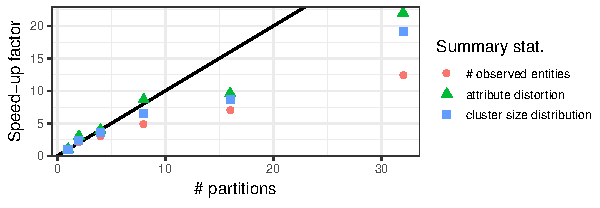
\includegraphics{plot-partitions-speed-up-aws.pdf}
  \caption{Efficiency of \dblink\ as a function of the
    number of blocks $B$ and summary statistic of interest 
    (larger is better).
    The speed-up measures the ESS rate relative to the ESS rate 
    for $B = 1$ (no partitioning) for the \texttt{NLTCS} data set.}
  \label{app-fig:speed-up-vs-num-partitions}
\end{figure}

\begin{figure}
  \centering
  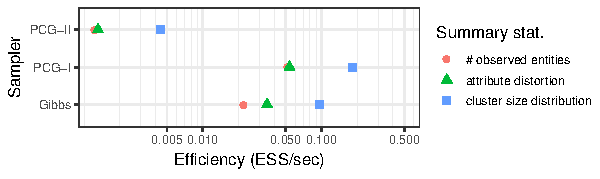
\includegraphics{plot-sampler-speed-up-aws.pdf}
  \caption{Efficiency of \dblink\ as a function of the 
    sampler and summary statistic of interest (larger is better).
    All measurements are for the \texttt{NLTCS} data set with 
    $B = 16$.
    }
  \label{app-fig:speed-up-vs-sampler}
\end{figure}

\section{Balance of the blocks}
\label{app-sec:balance-partitions}
In Section~\ref{sec:kd}, we proposed a blocking function based on $k$-d 
trees, and argued that it could yield balanced blocks with good entity 
separation.
While running \dblink\ with the $k$-d tree blocking function, we recorded the 
size of the blocks ($|\partset_{b}|$ for all $b$) to assess whether 
they were well-balanced.
Figure~\ref{app-fig:partition-sizes} illustrates the results in terms of the 
relative absolute deviation from the perfectly balanced configuration
(where the entities are divided equally among the blocks). 
We can see that the $k$-d tree partitioner is functioning quite well---the 
deviation from the perfectly balanced configuration is no more than 10\% for 
all data sets.

\begin{figure}
  \centering
  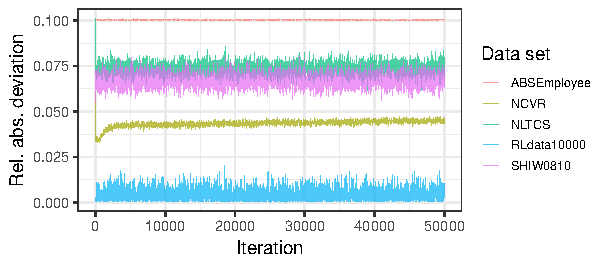
\includegraphics{partition-sizes-plot.pdf}
  \caption{Balance of the blocks for a single run on each
    data set.
    The balance is measured in terms of the relative absolute 
    deviation from the perfectly balanced configuration.
    The number of blocks $B = 64, 64, 16, 2, 8$ for each data set (in the 
    order listed in the legend).
  }
  \label{app-fig:partition-sizes}
\end{figure}

\section{Uncertainty measures}
\label{app-sec:error-num-ents}
\dblink\ allows for measures of uncertainty to be reported, unlike the 
baseline methods, since we have the full posterior distribution.
For example, in Figure~\ref{app-fig:error-num-ents} we compute posterior estimates 
for the number of entities present in each data set, with 95\% 
Bayesian credible intervals.
Note that the posterior estimates are typically quite 
sharp.
This seems to confirm arguments by~\citet{steorts_bayesian_2016} 
regarding the informativeness of the prior for the linkage 
structure in \blink. 
Research on less informative priors is ongoing~\citep{zanella_flexible_2016}.

\begin{figure}
  \centering
  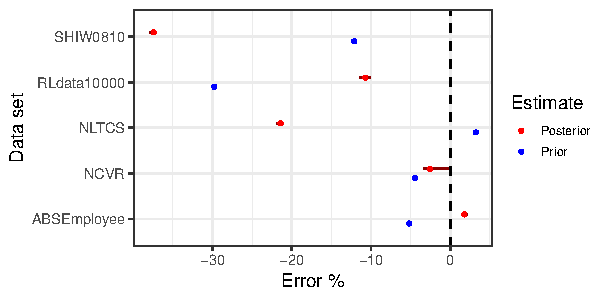
\includegraphics{posterior-bias-plot-dark.pdf}
  \caption{Percentage error in the posterior\slash prior estimates for the 
    number of observed entities for \dblink.
    The posterior estimates are generally sharp and underestimate the true 
    number of observed entities.
  }
  \label{app-fig:error-num-ents}
\end{figure}

%\color{blue}
\section{Sensitivity analysis}
\label{app-sec:sensitivity}
We conducted an empirical sensitivity analysis for \dblink\ 
using the \texttt{RLdata10000} data set.
We selected this data set as it is relatively small, which made it 
quick to run the inference for various hyperparameter combinations.
The parameters tested were:
\begin{itemize}
  \item $\alpha_\ell, \beta_\ell$: the shape parameters for the Beta prior on 
  the distortion probabilities. 
  We used the same values for all attributes ($a$). 
  \item $E$: the size of the latent population.
  \item $s_{\mathrm{max}}$: the scaling factor for the similarity function. 
  This controls the inverse temperature of the softmax distribution for the 
  distorted attribute values. 
\end{itemize}
We varied each of these parameters in turn, while holding all other parameters 
fixed.
For the Beta prior on the distortion probabilities, we first varied the 
strength while fixing the prior mean to $\sim 1\%$, then we varied the mean 
(1\%, 5\% and 10\%) while fixing $\alpha + \beta$ (related to the strength). 
Table~\ref{tbl:sensitivity} presents the evaluation measures for each 
combination of parameters.
The results indicate that the inferred linkage structure is relatively 
sensitive to all of the parameters, however sensitivity is in general 
predictable, following clear and intuitive trends.
Of particular interest is the fact that the model performs best when the 
Beta prior on the distortion probabilities is sharply peaked near zero. 
It seems that the model has a tendency to overestimate the amount of 
distortion, particularly in the absence of ground truth.

\begin{table}
	\centering
  \caption{Sensitivity analysis for various parameters combinations 
  using \texttt{RLdata10000}. The first group of rows tests the effect of 
  varying the \emph{strength} of the Beta prior, the second group tests the 
  effect of varying the \emph{mean} of the Beta prior, the third group 
  tests the effect of varying the population size, and the fourth group 
  tests the effect of varying the scaling factor for the similarity function.}
	\label{tbl:sensitivity}
	\spacingset{1}
  \footnotesize
  \begin{center}
	\begin{tabular}{*{9}{c}}
		\toprule
		\multicolumn{2}{c}{Distortion} & Pop.\ size & Max.\ sim. & \multicolumn{3}{c}{Pairwise measures} & \multicolumn{2}{c}{Cluster measures} \\
		\cmidrule(lr){1-2} \cmidrule(lr){3-3} \cmidrule(lr){4-4} \cmidrule(lr){5-7} \cmidrule(lr){8-9}
		$\alpha$       & $\beta$          & $E$            & $s_{\mathrm{max}}$ & Precision & Recall & F1-score & ARI & Err. \# clust.\ \\
		\midrule 
    \textbf{0.1}   & \textbf{10.0}    & 10000          & 10.0          & 0.5342 & 0.9990 & 0.6962 & 0.6962 & $-17.47\%$ \\
    \textbf{1.0}   & \textbf{100.0}   & 10000          & 10.0          & 0.5435 & 0.9990 & 0.7040 & 0.7040 & $-16.58\%$ \\
    \textbf{10.0}  & \textbf{1000.0}  & 10000          & 10.0          & 0.6334 & 0.9970 & 0.7747 & 0.7747 & $-10.97\%$ \\
    \textbf{100.0} & \textbf{10000.0} & 10000          & 10.0          & 0.9180 & 0.9850 & 0.9503 & 0.9503 & $-1.595\%$ \\
    \midrule
    \textbf{10.0}  & \textbf{1000.0}  & 10000          & 10.0          & 0.6334 & 0.9970 & 0.7747 & 0.7747 & $-10.97\%$ \\
    \textbf{50.5}  & \textbf{959.5}   & 10000          & 10.0          & 0.6132 & 0.9970 & 0.7593 & 0.7593 & $-11.90\%$ \\
    \textbf{101.0} & \textbf{909.0}   & 10000          & 10.0          & 0.5992 & 0.9970 & 0.7485 & 0.7485 & $-12.90\%$ \\
    \midrule
    10.0           & 1000.0           & \textbf{9000}  & 10.0          & 0.5306 & 0.9970 & 0.6926 & 0.6926 & $-15.65\%$ \\
    10.0           & 1000.0           & \textbf{10000} & 10.0          & 0.6334 & 0.9970 & 0.7747 & 0.7747 & $-10.97\%$ \\
    10.0           & 1000.0           & \textbf{11000} & 10.0          & 0.6999 & 0.9960 & 0.8221 & 0.8221 & $-7.365\%$ \\
    \midrule
    10.0           & 1000.0           & 10000          & \textbf{5.0}  & 0.6927 & 0.9940 & 0.8164 & 0.8164 & $-22.12\%$ \\
    10.0           & 1000.0           & 10000          & \textbf{10.0} & 0.6334 & 0.9970 & 0.7747 & 0.7747 & $-10.97\%$ \\
    10.0           & 1000.0           & 10000          & \textbf{50.0} & 0.2112 & 0.3920 & 0.2745 & 0.2745 & $-12.50\%$ \\
		\bottomrule
  \end{tabular}
  \end{center}
\end{table}


\section{Details of inference for the case study to the 2010 Decennial Census}
\label{app-sec:census-mcmc}
We ran inference for 15,000 iterations using the PCG-I sampler.
After removing 5,000 iterations as burn-in and applying thinning with 
an interval of 10, we obtained 1,000 approximate samples from the 
posterior.
Convergence diagnostics are consistent with those reported for 
the other data sets in Appendix~\ref{app-sec:trace-plots}, 
and are complicated to release due to the fact that the data is 
protected under Title~13. 
Releasing each iteration of a Gibbs sampler could potentially say something 
about individuals in the population, and thus, for privacy reasons, these 
diagnostics are omitted.


\pagebreak
\section{Trace plots}
\label{app-sec:trace-plots}
\subsection{Attribute-level distortion}
The following figures relate to the aggregate distortion per attribute 
for each data set.
On the left are the trace plots, which show the aggregate distortion 
for each attribute (stacked vertically) along the Markov chain.
On the right are the corresponding autocorrelation plots.

\begin{figure}[H]
  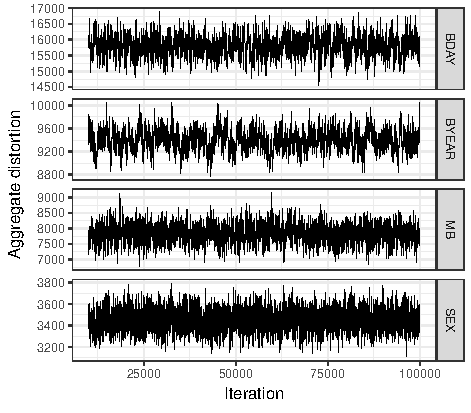
\includegraphics[width=0.48\linewidth]{ABSEmployee_attribute-distortions} \hfill
  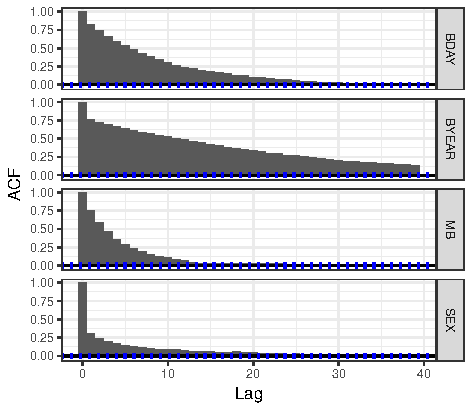
\includegraphics[width=0.48\linewidth]{ABSEmployee_attribute-distortions-acf}
  \caption{Attribute-level distortion for \texttt{ABSEmployee}}
\end{figure}
\begin{figure}[H]
  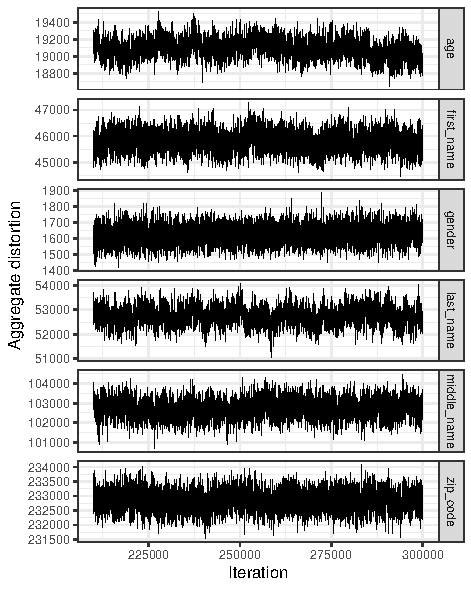
\includegraphics[width=0.48\linewidth]{NCVR_attribute-distortions} \hfill
  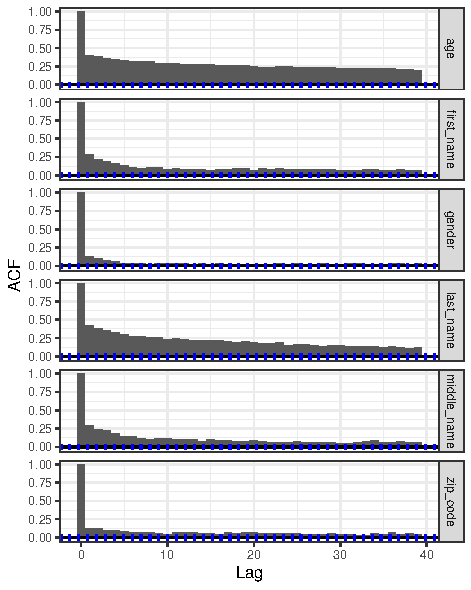
\includegraphics[width=0.48\linewidth]{NCVR_attribute-distortions-acf}
  \caption{Attribute-level distortion for \texttt{NCVR}}
\end{figure}
\begin{figure}[H]
  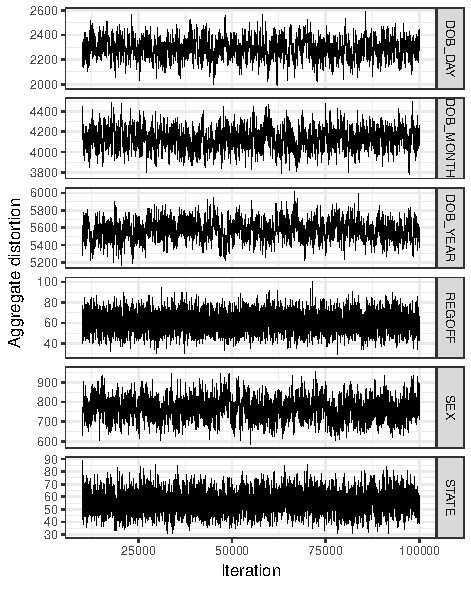
\includegraphics[width=0.48\linewidth]{NLTCS_attribute-distortions} \hfill
  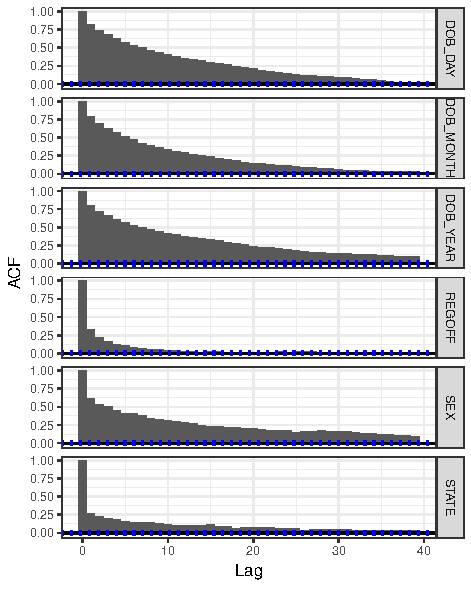
\includegraphics[width=0.48\linewidth]{NLTCS_attribute-distortions-acf}
  \caption{Attribute-level distortion for \texttt{NLTCS}}
\end{figure}
\begin{figure}[H]
  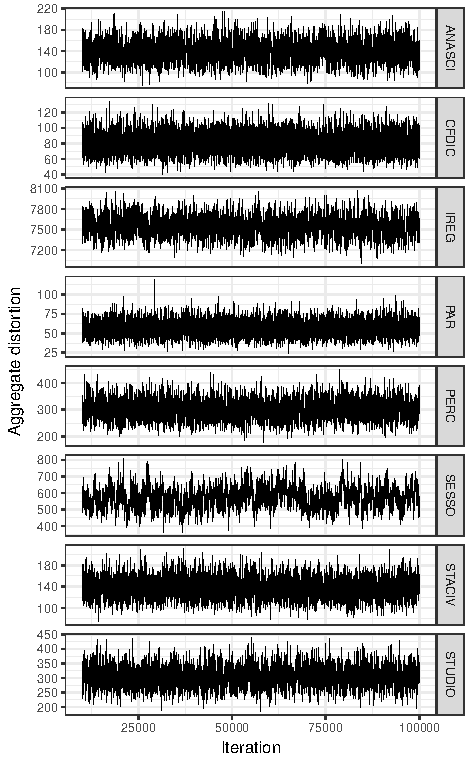
\includegraphics[width=0.48\linewidth]{SHIW_attribute-distortions} \hfill
  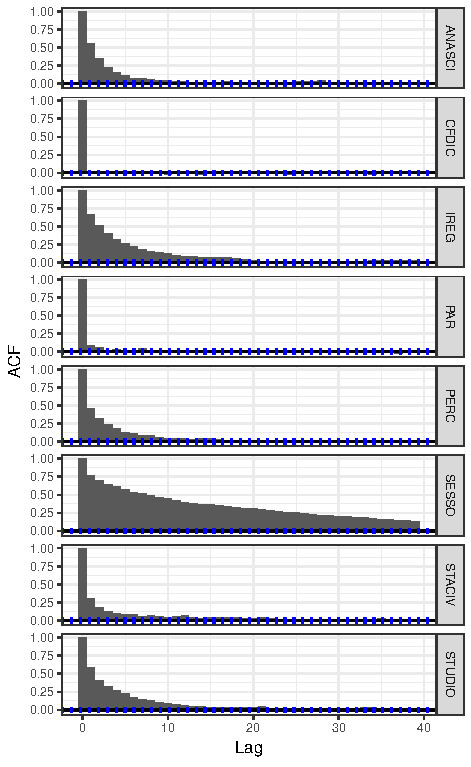
\includegraphics[width=0.48\linewidth]{SHIW_attribute-distortions-acf}
  \caption{Attribute-level distortion for \texttt{SHIW0810}}
\end{figure}
\begin{figure}[H]
  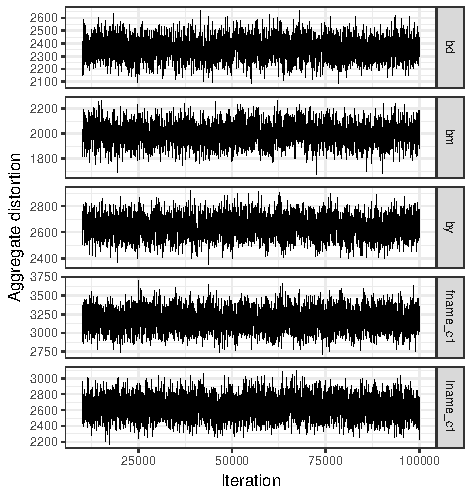
\includegraphics[width=0.48\linewidth]{RLdata10000_attribute-distortions} \hfill
  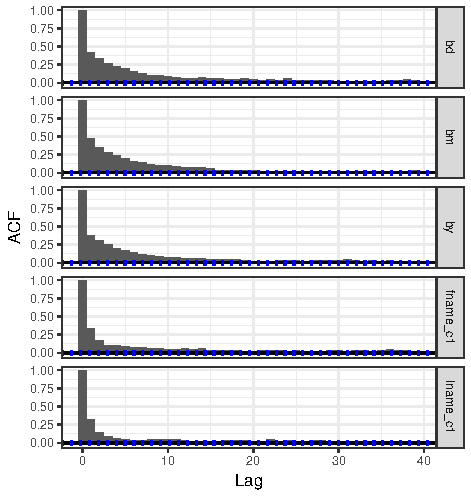
\includegraphics[width=0.48\linewidth]{RLdata10000_attribute-distortions-acf}
  \caption{Attribute-level distortion for \texttt{RLdata10000}}
\end{figure}

\subsection{Distribution of record distortion}
The following figures relate to the distribution of record distortion 
for each data set.
Specifically, we count the number of records with 0 distorted attributes, 
1 distorted attribute, 2 distorted attributes, etc.
On the left are the trace plots, which show the record counts for each 
distortion level (stacked vertically) along the Markov chain.
On the right are the corresponding autocorrelation plots.

\begin{figure}[H]
  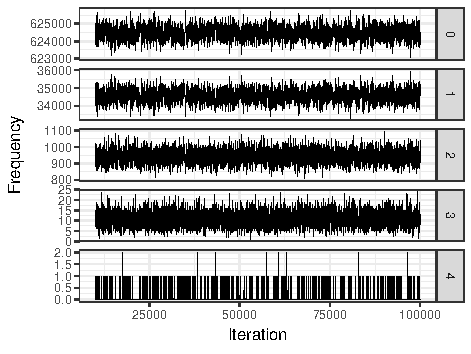
\includegraphics[width=0.48\linewidth]{ABSEmployee_record-distortions} \hfill
  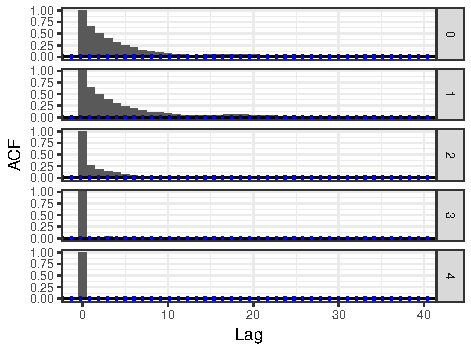
\includegraphics[width=0.48\linewidth]{ABSEmployee_record-distortions-acf}
  \caption{Distribution of record distortion for \texttt{ABSEmployee}}
\end{figure}
\begin{figure}[H]
  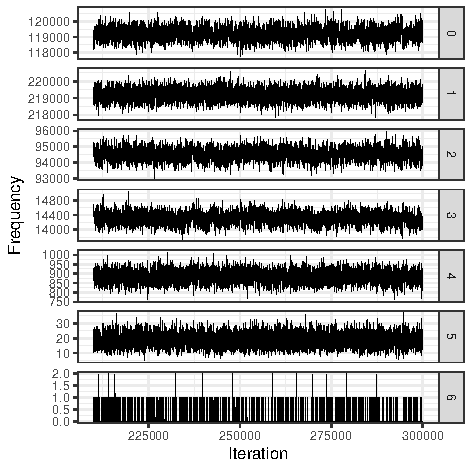
\includegraphics[width=0.48\linewidth]{NCVR_record-distortions} \hfill
  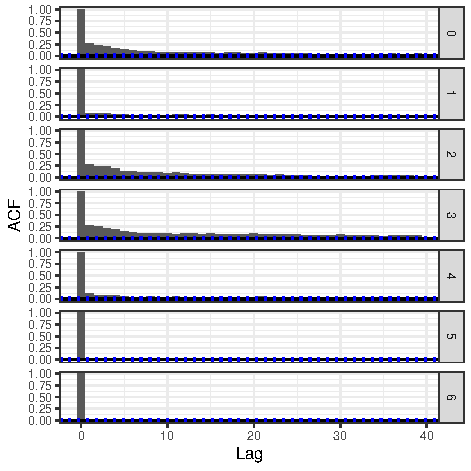
\includegraphics[width=0.48\linewidth]{NCVR_record-distortions-acf}
  \caption{Distribution of record distortion for \texttt{NCVR}}
\end{figure}
\begin{figure}[H]
  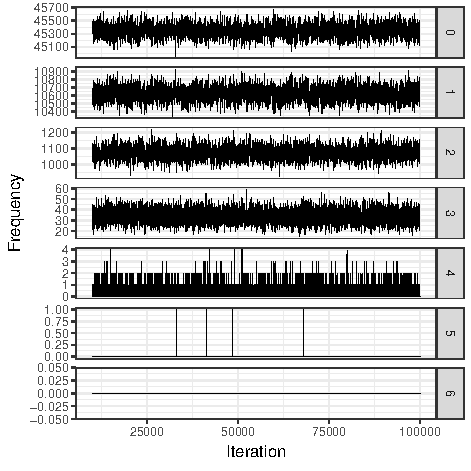
\includegraphics[width=0.48\linewidth]{NLTCS_record-distortions} \hfill
  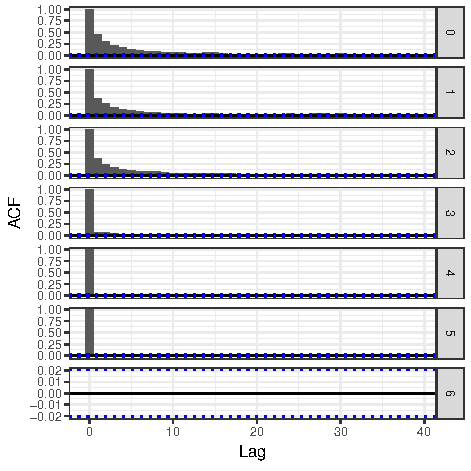
\includegraphics[width=0.48\linewidth]{NLTCS_record-distortions-acf}
  \caption{Distribution of record distortion for \texttt{NLTCS}}
\end{figure}
\begin{figure}[H]
  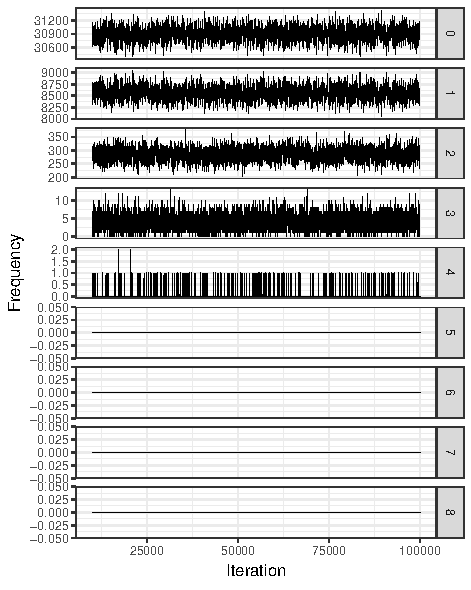
\includegraphics[width=0.48\linewidth]{SHIW_record-distortions} \hfill
  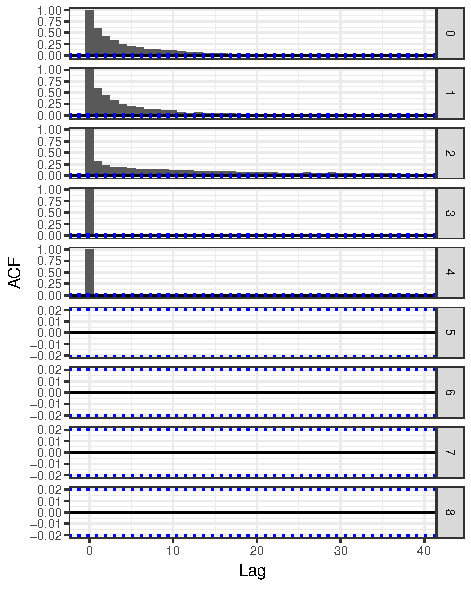
\includegraphics[width=0.48\linewidth]{SHIW_record-distortions-acf}
  \caption{Distribution of record distortion for \texttt{SHIW0810}}
\end{figure}
\begin{figure}[H]
  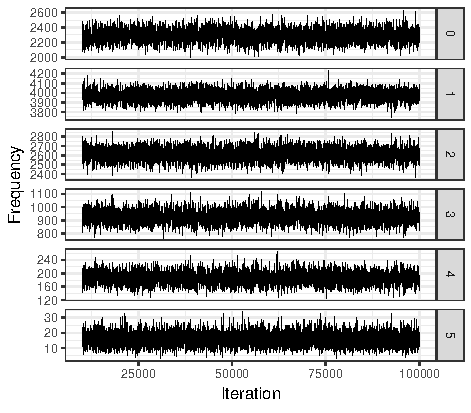
\includegraphics[width=0.48\linewidth]{RLdata10000_record-distortions} \hfill
  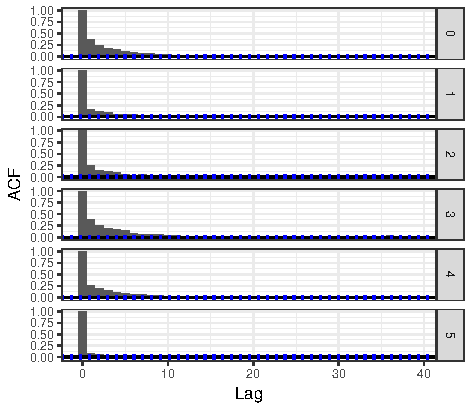
\includegraphics[width=0.48\linewidth]{RLdata10000_record-distortions-acf}
  \caption{Distribution of record distortion for \texttt{RLdata10000}}
\end{figure}

\subsection{Cluster size distribution}
The following figures relate to the distribution of cluster (entity) sizes 
for each data set.
Specifically, we count the number of entities with 0 linked records, 
1 linked record, 2 linked records, etc.
On the left are the trace plots, which show the counts for each cluster size 
(stacked vertically) along the Markov chain.
On the right are the corresponding autocorrelation plots.

\begin{figure}[H]
  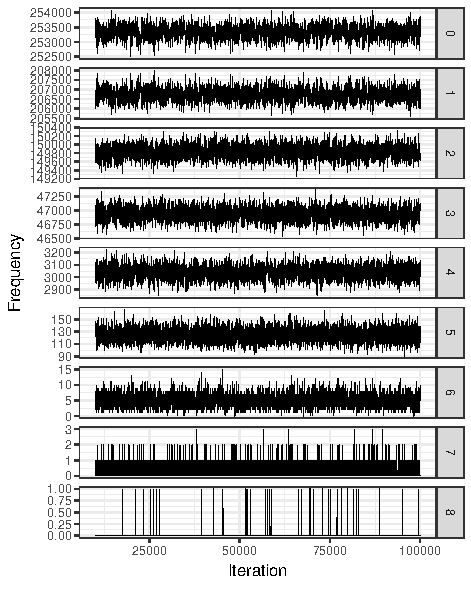
\includegraphics[width=0.48\linewidth]{ABSEmployee_cluster-size-distribution} \hfill
  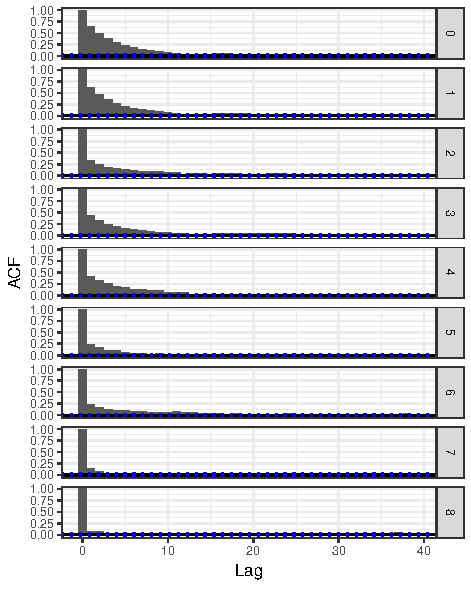
\includegraphics[width=0.48\linewidth]{ABSEmployee_cluster-size-distribution-acf}
  \caption{Cluster size distribution for \texttt{ABSEmployee}}
\end{figure}
\begin{figure}[H]
  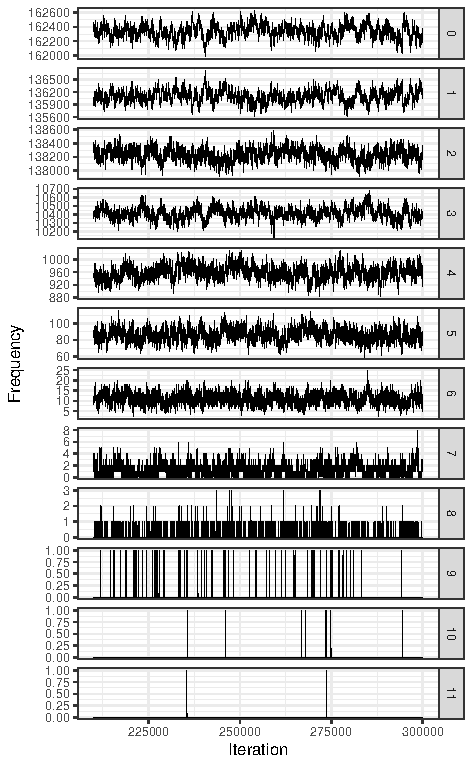
\includegraphics[width=0.48\linewidth]{NCVR_cluster-size-distribution} \hfill
  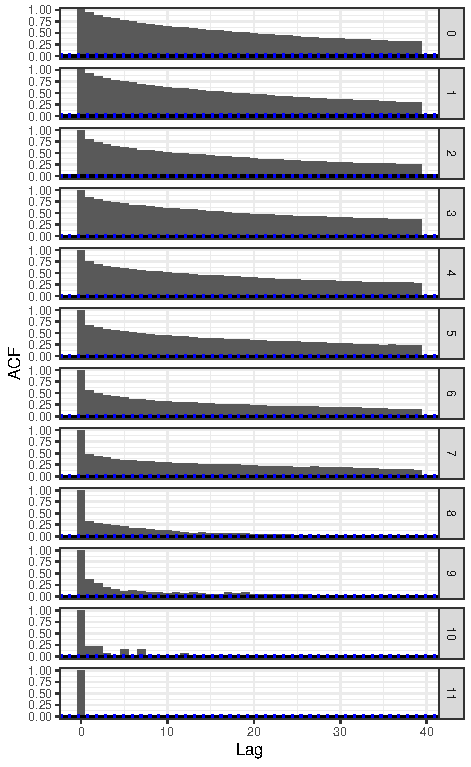
\includegraphics[width=0.48\linewidth]{NCVR_cluster-size-distribution-acf}
  \caption{Cluster size distribution for \texttt{NCVR}}
\end{figure}
\begin{figure}[H]
  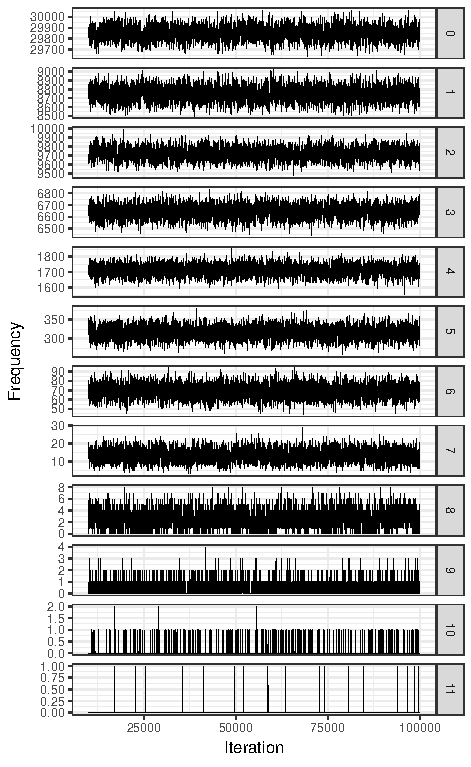
\includegraphics[width=0.48\linewidth]{NLTCS_cluster-size-distribution} \hfill
  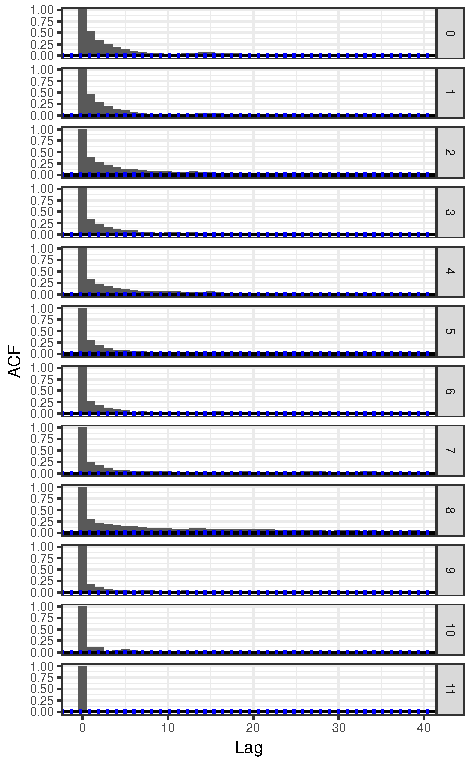
\includegraphics[width=0.48\linewidth]{NLTCS_cluster-size-distribution-acf}
  \caption{Cluster size distribution for \texttt{NLTCS}}
\end{figure}
\begin{figure}[H]
  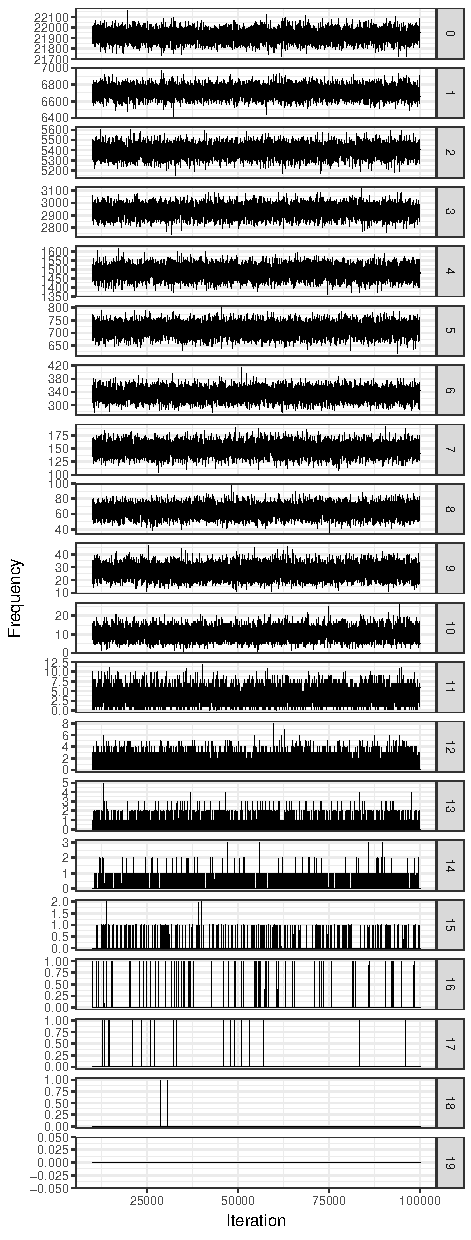
\includegraphics[width=0.48\linewidth]{SHIW_cluster-size-distribution} \hfill
  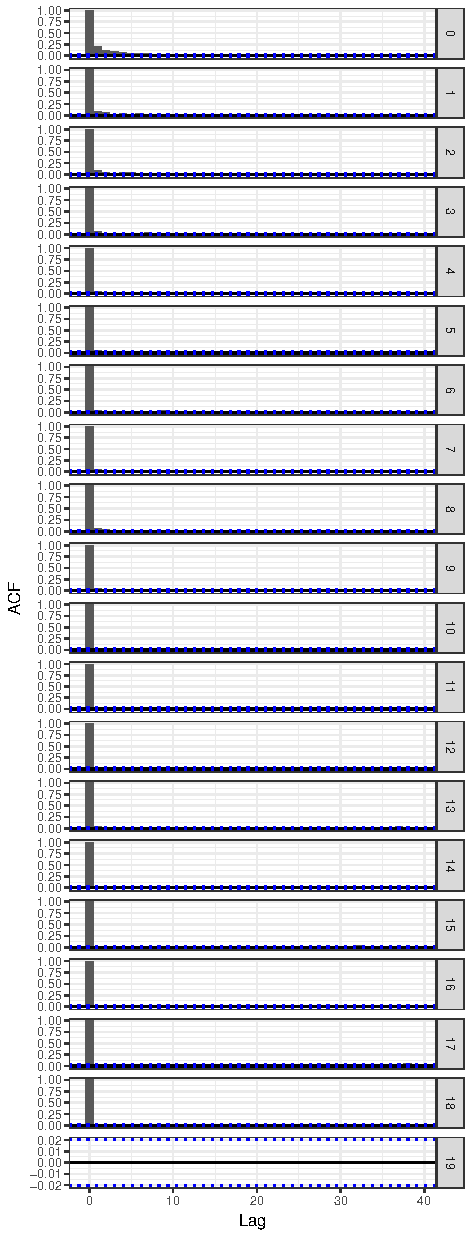
\includegraphics[width=0.48\linewidth]{SHIW_cluster-size-distribution-acf}
  \caption{Cluster size distribution for \texttt{SHIW0810}}
\end{figure}
\begin{figure}[H]
  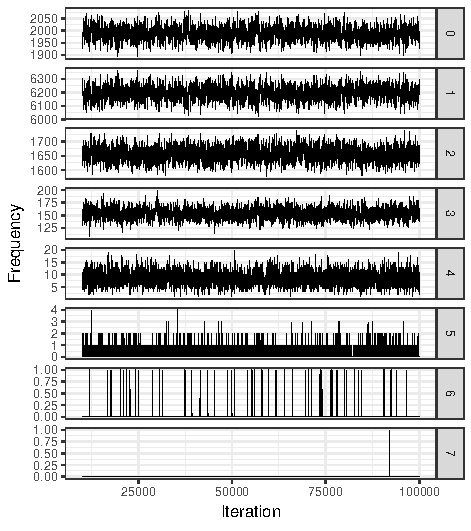
\includegraphics[width=0.48\linewidth]{RLdata10000_cluster-size-distribution} \hfill
  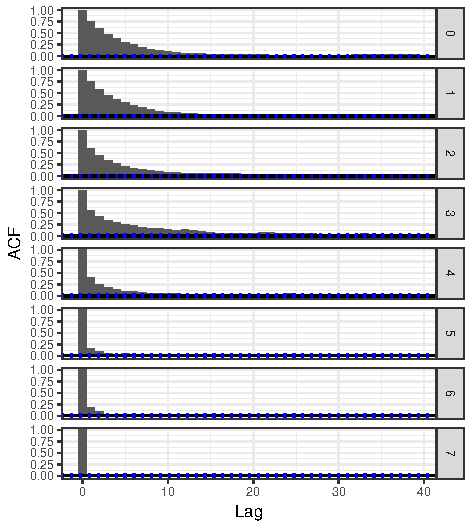
\includegraphics[width=0.48\linewidth]{RLdata10000_cluster-size-distribution-acf}
  \caption{Cluster size distribution for \texttt{RLdata10000}}
\end{figure}

%\let\noopsort\undefined
%\let\printfirst\undefined
%\let\singleletter\undefined
%\let\switchargs\undefined
{
\footnotesize
\bibliographystyle{jasa}
\bibliography{dblink}
}

\end{document}
